\begin{frame}
    \frametitle{Trường vector}
    \begin{columns}
        \column{0.5\textwidth}
            \begin{figure}
                \centering
                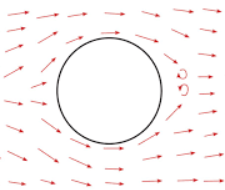
\includegraphics[width=4cm, height=3cm]{Content/Figure/streamline.png}
                \caption{Trường vận tốc của chất lưu}
            \end{figure}
            \[\mathbf{v}=\mathbf{v}(x,y)=\mathbf{v}(r,\theta)\]
        \column{0.5\textwidth}
            \begin{figure}
                \centering
                
\includegraphics[width=4cm, height=3cm]{Content/Figure/electric_charge.png}
                \caption{Trường tĩnh điện của điện tích điểm}
            \end{figure}
            \[\mathbf{E}=\mathbf{E}(x,y,z)=\mathbf{E}(r)\]
    \end{columns}
\end{frame}
\begin{frame}
    \frametitle{Trường (lực) thế}
    \begin{enumerate}
        \item Giá trị của tích phân đường (công) chỉ phụ thuộc vào điểm đầu và điểm cuối: \[-\int_{\mathbf{r}_1}^{\mathbf{r}_2}\mathbf{F}\cdot\text{d}\mathbf{l}=V(\mathbf{r}_1)-V(\mathbf{r}_2).\]
        \item Lưu số trên một đường cong kín là bằng không: \[\oint_{\mathcal{C}}\mathbf{F}\cdot\text{d}\mathbf{l}=0.\]
        \item Trường lực thế có thể biểu diễn dưới dạng gradient của một hàm vô hướng: \[\mathbf{F}=-\nabla V.\]
    \end{enumerate}
    \vspace{-5pt}

    Ví dụ về các lực thế: lực hấp dẫn, lực đàn hồi, \dots
\end{frame}
\begin{frame}
    \frametitle{Quan hệ giữa các tính chất của trường thế}
    \begin{columns}
        \begin{column}{0.5\textwidth}
            \scriptsize
            Từ tính chất thứ nhất,
            \[-\mathbf{F}\cdot\text{d}\mathbf{l}=\text{d}V.\]
            Do đó,
            \[-(F_x \text{d}x +F_y \text{d}y +F_z \text{d}z)=\partial_x V\text{d}x +\partial_y V\text{d}y +\partial_z V\text{d}z.\]
            Đồng nhất hai vế, 
            \[\mathbf{F}=-\nabla V.\]
        \end{column}
        \begin{column}{0.5\textwidth}
            \scriptsize
            Từ tính chất thứ hai (xét trên mặt phẳng \(xy\)),
            \begin{figure}
                \centering
                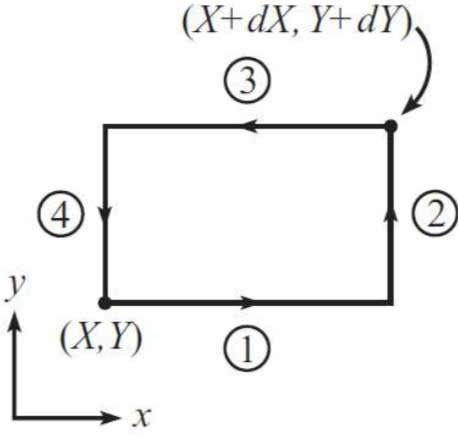
\includegraphics[width=3.5cm, height=3cm]{Content/Figure/Curl.jpg}
            \end{figure}
            \[\oint \mathbf{F}\cdot \text{d}\mathbf{l}=\text{d}X\text{d}Y\left(\partial_x F_y -\partial_y F_x\right)=0.\]
            Tương tự cho các mặt phẳng khác,
            \vspace{-5pt}
            \begin{align*}
                &\text{d}Y\text{d}Z\left(\partial_y F_z -\partial_z F_y\right)=0.&\\
                &\text{d}X\text{d}Z\left(\partial_z F_x -\partial_x F_z\right)=0.&
            \end{align*}
        \end{column}
    \end{columns}
\end{frame}
\begin{frame}
    \frametitle{Curl và định lý Curl(Stokes)}
    \begin{columns}
        \begin{column}{0.5\textwidth}
            \scriptsize
            Curl của \(\mathbf{F}\) được định nghĩa là
            \[\nabla\times\mathbf{F}\equiv \det\left(\begin{bmatrix}
                \hat{x} & \hat{y} & \hat{z}\\
                \partial_x & \partial_y & \partial_z\\
                F_x & F_y & F_z
            \end{bmatrix}\right).\]
            Định lý Stokes tổng quát hoá cho mọi bề mặt:
            \begin{equation*}
                \int_{\mathcal{S}}(\nabla\times\mathbf{F})\cdot\text{d}\mathbf{a}=\oint_{\mathcal{C}}\mathbf{F}\cdot\text{d}\mathbf{l}.
            \end{equation*}
            Chú ý, \(\mathcal{C}\) là đường biên của bề mặt \(\mathcal{S}\).
        \end{column}
        \begin{column}{0.5\textwidth}
            \scriptsize
            Curl của một trường thế bằng không nên \(\mathbf{F}\) phải có dạng \(-\nabla V\) vì
            \[\nabla\times(\nabla V)=0 \quad\forall V.\]
            Cụ thể,
            \begin{align*}
                \partial_{xy}V=&\partial_{yx}V,\\
                \partial_{yz}V=&\partial_{zy}V,\\
                \partial_{zx}V=&\partial_{xz}V.   
            \end{align*}
            Tóm lại, điều kiện cần và đủ của một trường thế là \[\nabla\times \mathbf{F}=\mathbf{0}.\]
        \end{column}
    \end{columns}
\end{frame}
\begin{frame}
    \frametitle{Minh hoạ cho dòng chảy xoáy}
    \begin{columns}
        \begin{column}{0.5\textwidth}
            \begin{figure}
                \centering
                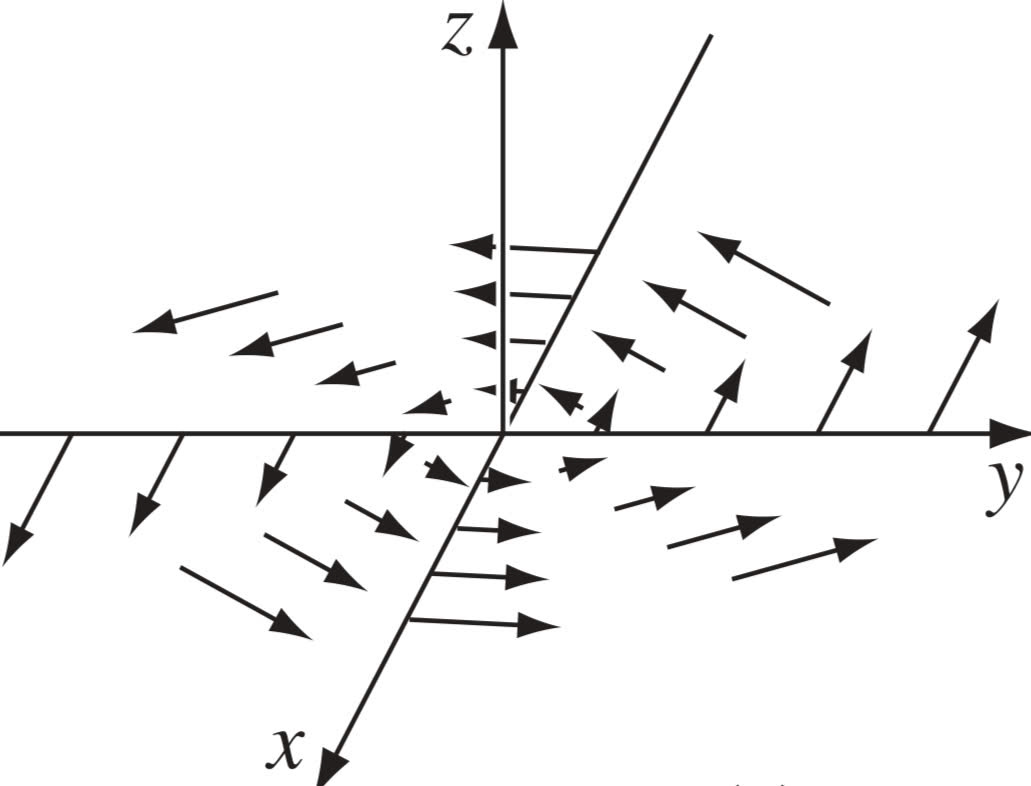
\includegraphics[width=4cm, height=3cm]{Content/Figure/illustration for curl.jpg}
            \end{figure}
            \[\mathbf{v}=-y\hat{x}+x\hat{y},\]
            \[\nabla\times\mathbf{v}=2\hat{z}.\]
        \end{column}
        \begin{column}{0.5\textwidth}
            \begin{figure}
                \centering
                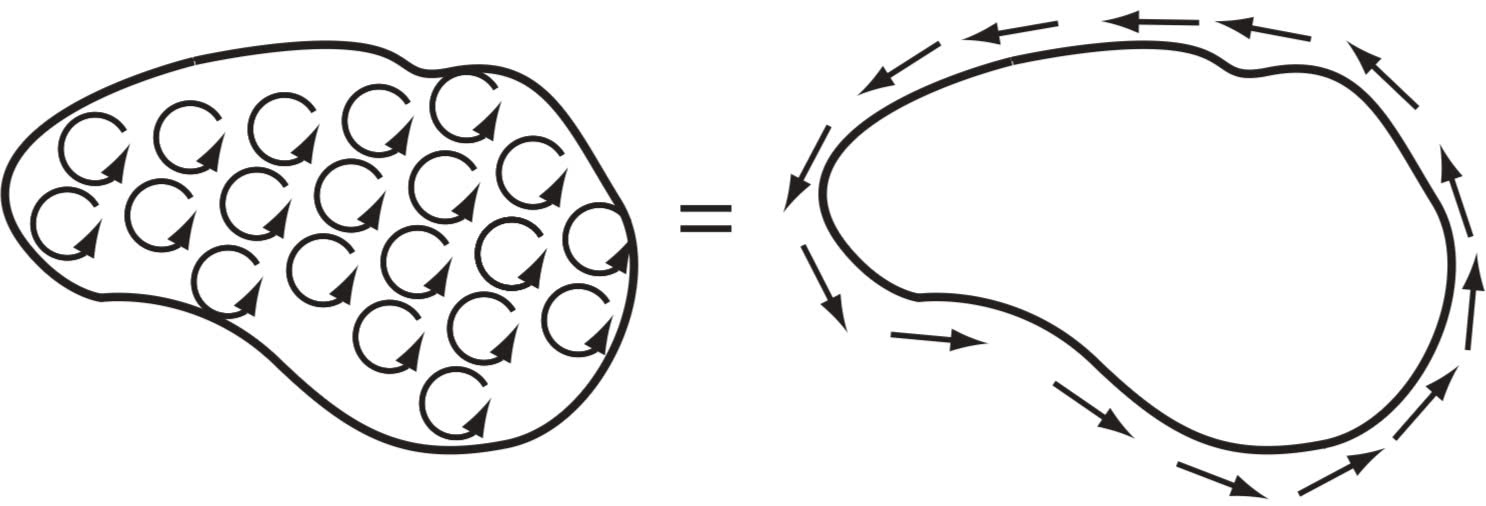
\includegraphics[width=4cm, height=2cm]{Content/Figure/illustration for Stoke.jpg}
                \caption{Định lý Stokes}
            \end{figure}
            \vspace{-8pt}

            \begin{figure}
                \centering
                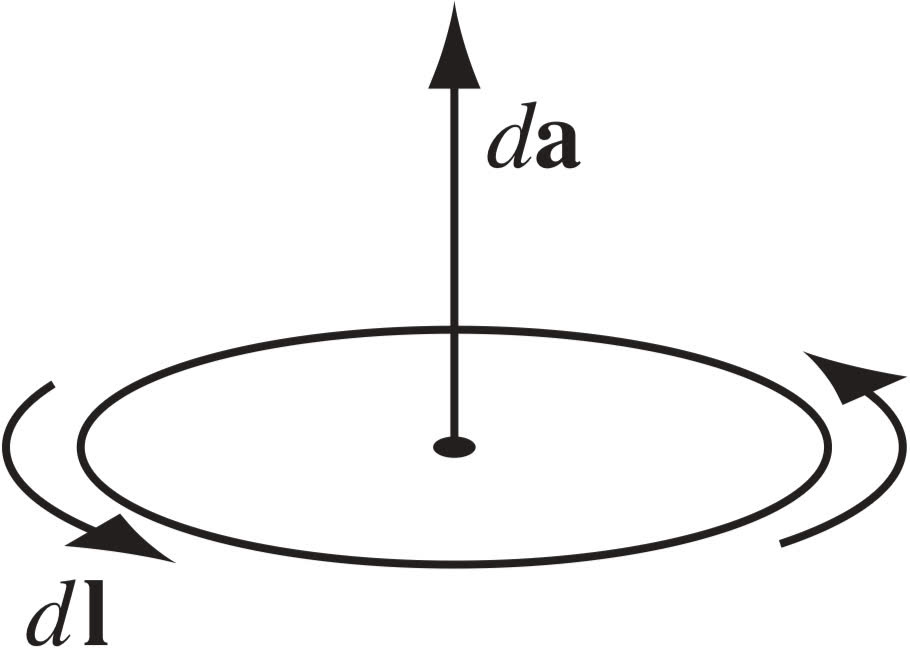
\includegraphics[width=2.5cm, height=2cm]{Content/Figure/direction_of_normal_vector.jpg}
                \caption{Chiều của vector pháp tuyến}
            \end{figure}
        \end{column}
    \end{columns}
\end{frame}